\chapter{\evaluation}
\label{chp:5}

Ebben a fejezetben kiértékelem munkámat mialatt megválaszolom a következő kérdéseket:

\begin{itemize}
	\item \textbf{Kérdés1}: Hogy aránylik egymáshoz az előfeldolgozás, a generálás és az utófeldolgozás időtartama?
	\item \textbf{Kérdés2}: Hogy skálázódik a generálás lekérdezés méretének szempontjából?
	\item \textbf{Kérdés3}: Hogy skálázódik a generálás lekérdezés darabszámának szempontjából?
	\item \textbf{Kérdés4}: Mennyire diverzek a lekérdezések a tesztelés minőségének szempontjából?
	\item \textbf{Kérdés5}: Milyen eredménnyel futtathatóak a lekérdezések egy Neo4j gráfadatbázison?
\end{itemize}

\section{Mérési környezet felállítása}


A méréseket eclipse fejlesztői környezetben végeztem. Ahhoz, hogy bemelegítsem a modell generátort memóriakezelés és optimalizálás szempontjából 5 extra futást adtam hozzá minden kiértékelt mérés előtt, melyek futásidejét a mérés során figyelmen kívül hagytam. A mérésekhez a generátor számára 4000 MB memóriát biztosítottam, és ez mindig elegendőnek bizonyult. Az összes mérést egy egyszerű asztali számítógépen végeztem (Intel Core i7-3520M CPU, 2.90GHz, Windows 10 Pro). A generáláshoz részmodellként egy 22 elemből álló ASG-t adtam meg, de csak az esszenciális részletek specifikálásával. Erre az alapra építve két különböző mérési környezetet implementáltam, hogy mind a 4 kérdésre választ tudjak adni. A két környezetben generált gráfok elkészültük után egy utófeldolgozás fázison mentek keresztül, ahol Cypher nyelvű lekérdezésekké fordítottam le őket.

\subsection{M1: Skálázódás modellkészlet méretében}

Az első mérési környezetben 50-50 eltérő lekérdezést generáltam, úgy, hogy 10 20 és 30 elemmel egészítettem ki a kiindulási állapotot. Minden mérést 10-szer megismételtem (a belemelegedést leszámolva). Az elrendezés célja, hogy a generátor skálázhatóságát vizsgálja modellkészlet méretének szempontjából.

\subsection{M2: Skálázódás modellkészlet méretében} 
A második  mérési környezetben 10-10 eltérő lekérdezést generáltam, 5, 10 ,15, ...,50, 100, 150, 200 elemmel egészítettem ki a kiindulási állapotot. Minden mérést 10-szer megismételtem (a belemelegedést leszámolva). Az elrendezés célja, hogy a generátor skálázhatóságát vizsgálja modellek méretének szempontjából.


\section{A futásidő összetétele}

\begin{figure}[htp]
	\centering
	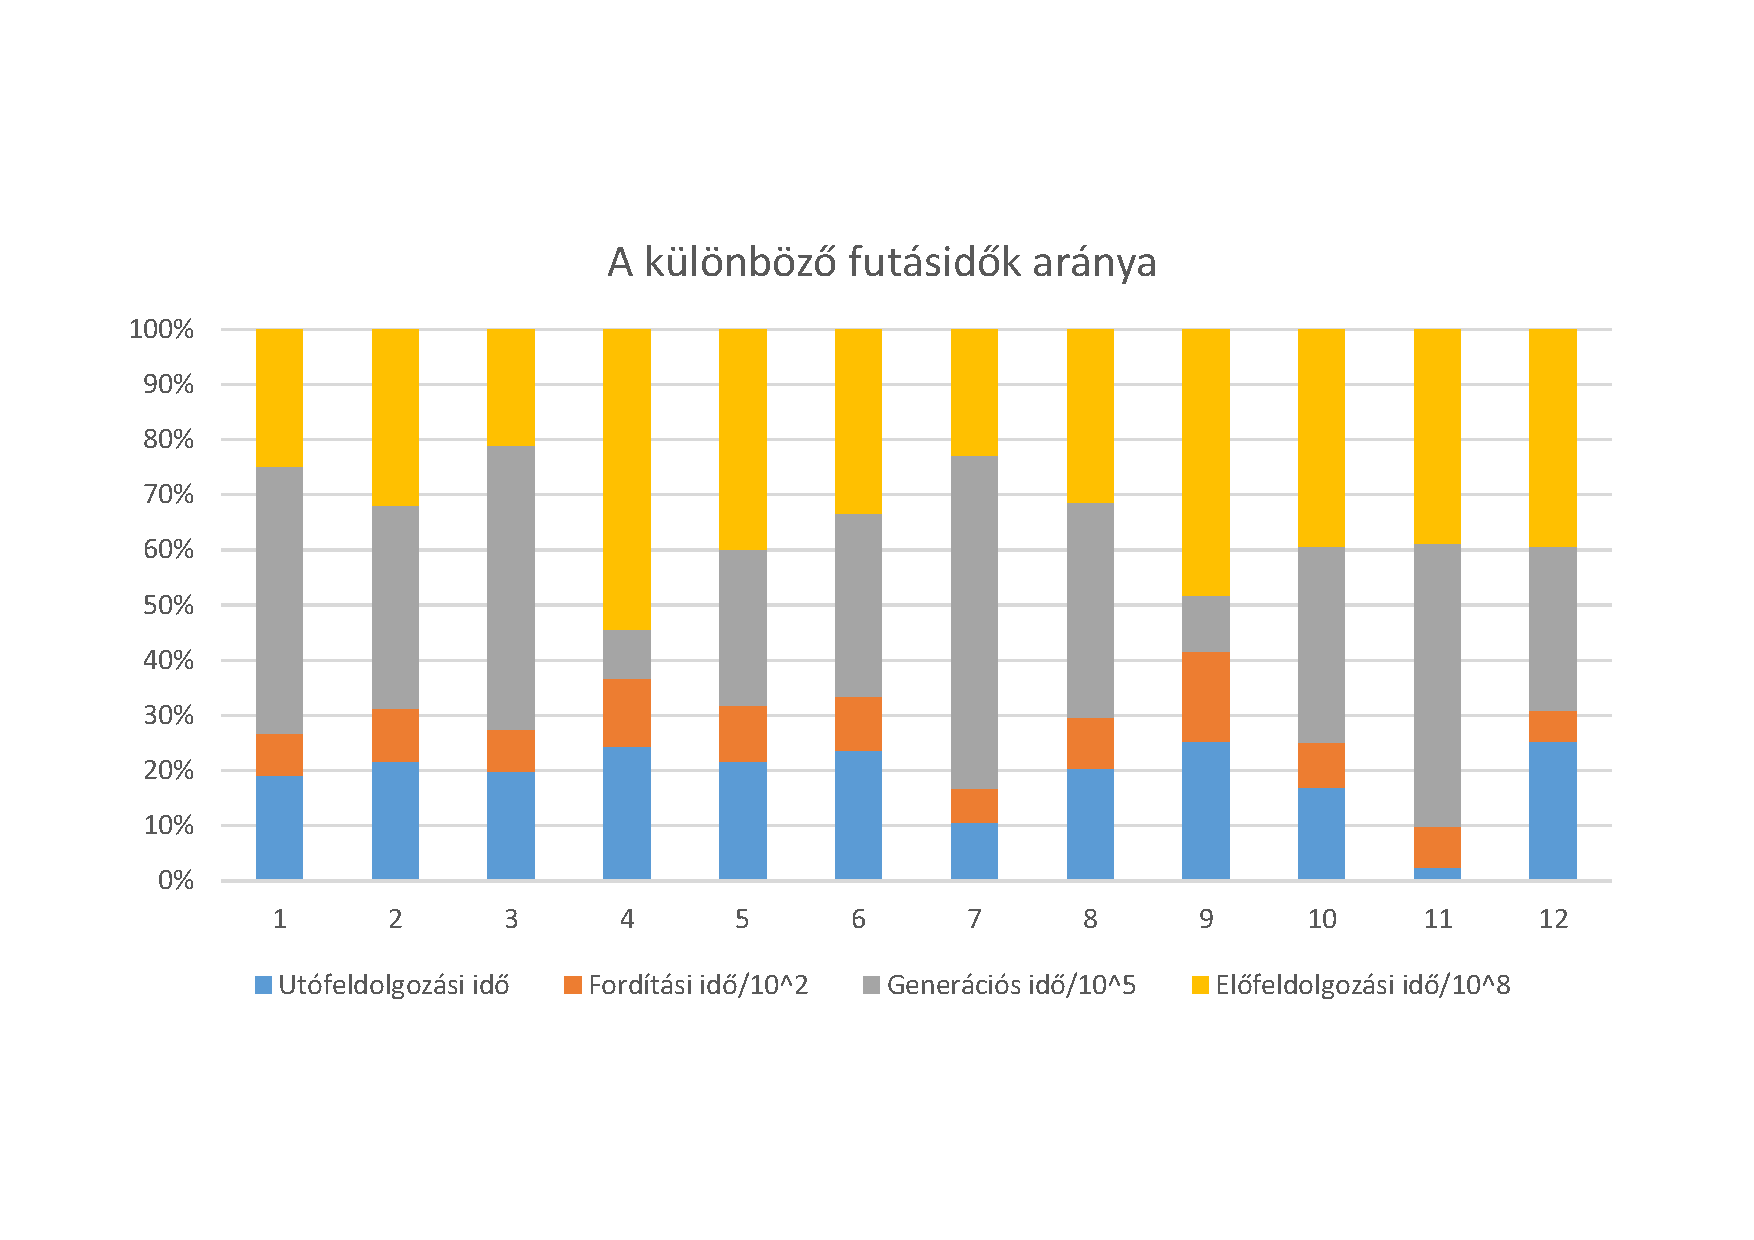
\includegraphics[width=1\textwidth]{figures/aránygrafikontáblázathelyett}
	\caption{A K1 mérés eredményei}
	\label{fig:grafikon}
\end{figure}

A futásidő összetételének vizsgálatát az M1 mérési környezetben végeztem el, de M2 esetén is hasonló karakterisztikát mutat. A mérés eredményei  \aref{fig:grafikon}. ábrán láthatóak. Az ábra segítségével azt szeretném bemutatni, hogy a különböző futásidők nagyságrendileg mekkora részét képezik a futásidő egészének. A három szín három értéket reprezentál: az előfeldolgozás idejét (ide tartozik a modellezési nyelv beolvasása, leképezése logikai feltételekké, a logikai probléma megfelelő formára hozása) kék színnel, a generálás idejét (ide a VIATRA Solver futása tartozik) szürke színnel, az utófeldogozás idejét (logikai probléma értelmezése, gráfként való ábrázolása, utófeldolgozás, változók és literálok elnevezése, végül a megoldás gráf ASG -ként való értelmezése és szöveggé alakítása) pedig narancssárga színnel jelölöm. (Alulról felfelé kék, szürke, narancs.) A grafikon vízszintes tengelye a teljes futásidőt mutatja meg. Az első oszlop a 10 a második a 20 a harmadik pedig a 30 hozzáadott csomópontban minimalizált al-környezetben végzett mérések futásidejének összegét ábrázolja. 

Az ábrán látható, hogy míg az elő és az utófeldolgozás összes ideje nem mutat jelentős különbséget a három esetben, addig a generálás időtartama szignifikánsan különbözik. Láthatóan a legkisebb méretnél a leghosszabb és a legnagyobbnál a legrövidebb. (Ennek az okát következő szekcióban fejtem ki.)

\textit{Végeredményben levonhatom a következtetést, hogy a futásidő leghosszabb részét a generálás ideje teszi ki, míg az előfeldolgozás és az utófeldolgozás arányaiban megegyező időtartamú, kisebb modellek esetében az előfeldolgozás, nagyobbak esetében pedig az utófeldolgozás tart tovább.}   

\section{Skálázódás a modellek méretének függvényében}

\begin{figure}[htp]
	\centering
	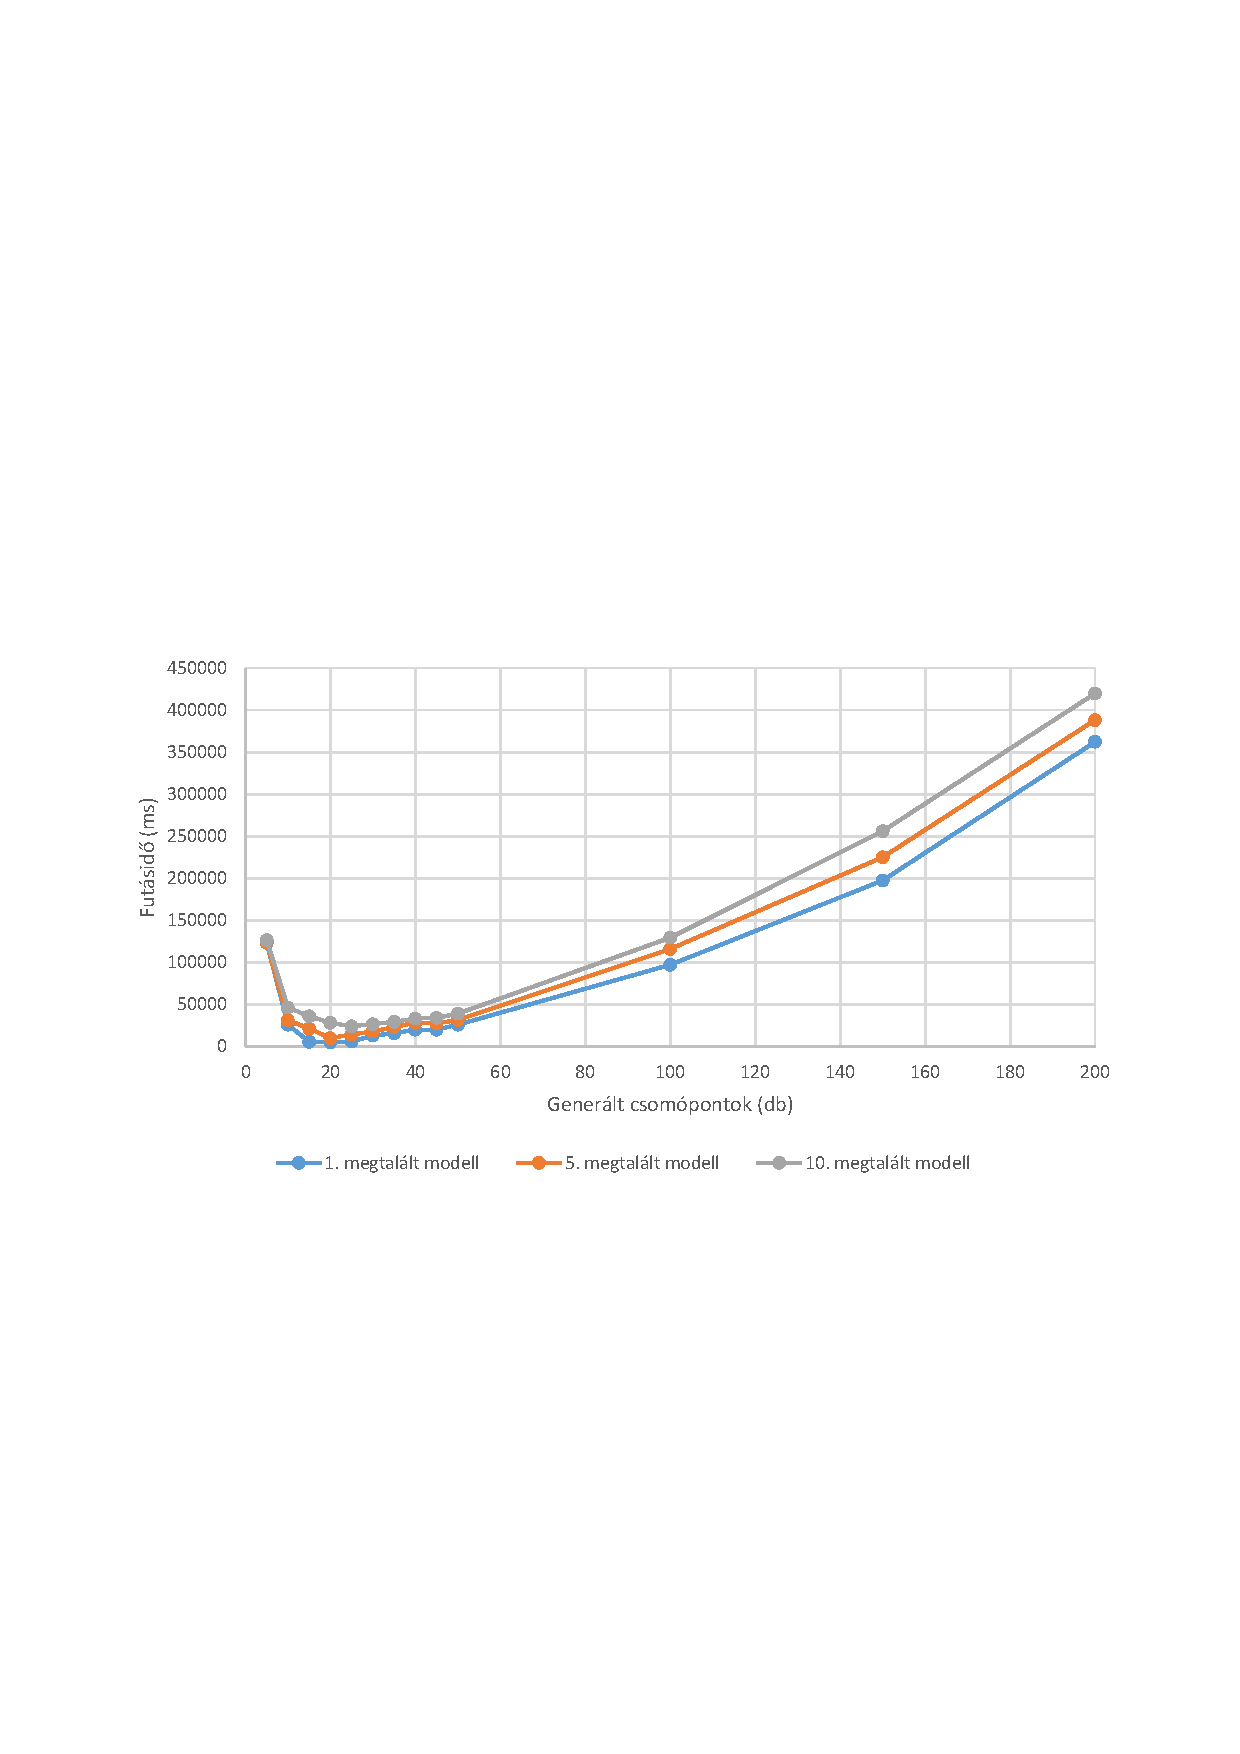
\includegraphics[width=1\textwidth]{figures/statisticsPlottal1}
	\caption{A K2 mérés eredményei}
	\label{fig:BmeresEredmeny}
\end{figure}

A második kérdésben felállított problémára az M2-es környezetben kerestem a választ. A mérés eredményei \aref{fig:BmeresEredmeny}. ábrán láthatóak. A következtetéseimet az 1., az 5. és a 10.modell megtalálásának  időpontjából vontam le. A 10 mérés során számolt futásidők mediánját ábrázoltam. A vízszintes tengelyen a hozzáadott csomópontok minimális elemszáma, míg a függőleges tengelyen az adott modell megtalálásához szükséges futásidő látható. 

Látható, hogy kis minimum darabszámú generált elem hozzáadásával nehezebben boldogult a generátor, mint a közepes elemszámokkal, ám a hatalmas modellek megtalálása is egyre nehezebb feladatnak bizonyult. A kis modelleknél mért lassúság azzal magyarázható, hogy a megadott részmodell elég nagy (22 elem), emiatt tovább kell keresgélni, hogy 10 hozzáadott elemből ki tudja-e tölteni az összes szükséges helyet, illetve ha nem tudja akkor növelnie kell a hozzáadott csomópontok számát, és újrapróbálkoznia. Nagyobb elemek esetén ez a probléma nem áll fenn, azonban a gráfgenerálás problémája egyenletesen növekszik.

A vizsgált alkalmazás nagyobb modelleknél négyzetes karakterisztikát mutat. A gráfgenerálás egy NP-nehéz probléma, így a négyzetes karakterisztika remek eredmény, de tetszőleges méretű lekérdezések elkészítésére nem biztos hogy alkalmas.

\textit{Tehát végeredményben állíthatom, hogy a generátor szépen oldja meg a problémát és 200 generált csomópontra még elfogadható futásidővel működik (10 percen belül). (\Aref{fig:examplequery} egy 200 csomópontból álló kifejezés látható illusztrációként). \Aref{fig:examplequery} lenti lekérdezés benchmarkolásra és tesztelésre is alkalmas hosszúságú.}

\begin{figure}[htp]
	\centering
	\begin{lstlisting}[style=cyphersmall]
	MATCH ( V1 : Semaphore { signal : "String1" } ) ,
	( V2 : Semaphore { position : "String2" , length : "String3" } ) ,
	( V3 : Region { id : "String4" , length : "String5" } ) ,
	( V4 : Semaphore { length : "String6" , active : "String7" } ) ,
	( V5 : Route { signal : "String8" , currentPosition : "String9" } )
	- [ V6 : requires { length : "String10" , position : "String11" } ] - 
	( V7 : Region { currentPosition : "String12" , length : "String13" } )
	- [ V8 : entry { signal : "String14" , active : "String15" } ] -
	( V9 : Route { active : "String16" , currentPosition : "String17" } ) ,
	( V10 : Segment { length : "String18" , signal : "String19" } ) ,
	( V11 : Semaphore { id : "String20" , active : "String21" } ) ,
	( V12 : Route { signal : "String22" } ) ,
	( V13 : Region { position : "String23" , signal : "String24" } ) ,
	( V14 : Region { currentPosition : "String25" , length : "String26" } ) ,
	( V15 : Route { currentPosition : "String27" , currentPosition : "String28" }),
	( V16 : Segment { currentPosition : "String29" , position : "String30" } ) ,
	( V17 : Switch { length : "String31" , currentPosition : "String32" } ) ,
	( V18 : Semaphore { id : "String33" , signal : "String34" } )
	RETURN V5 , V10 , V7 , V14 , V18 , V9 , V6 , V16
	\end{lstlisting}
	\caption{Példa lekérdezés}
	\label{fig:examplequery}
\end{figure}

\section{Skálázódás a modellek darabszámának függvényében}
 
\begin{figure}[htp]
	\centering                                                    
	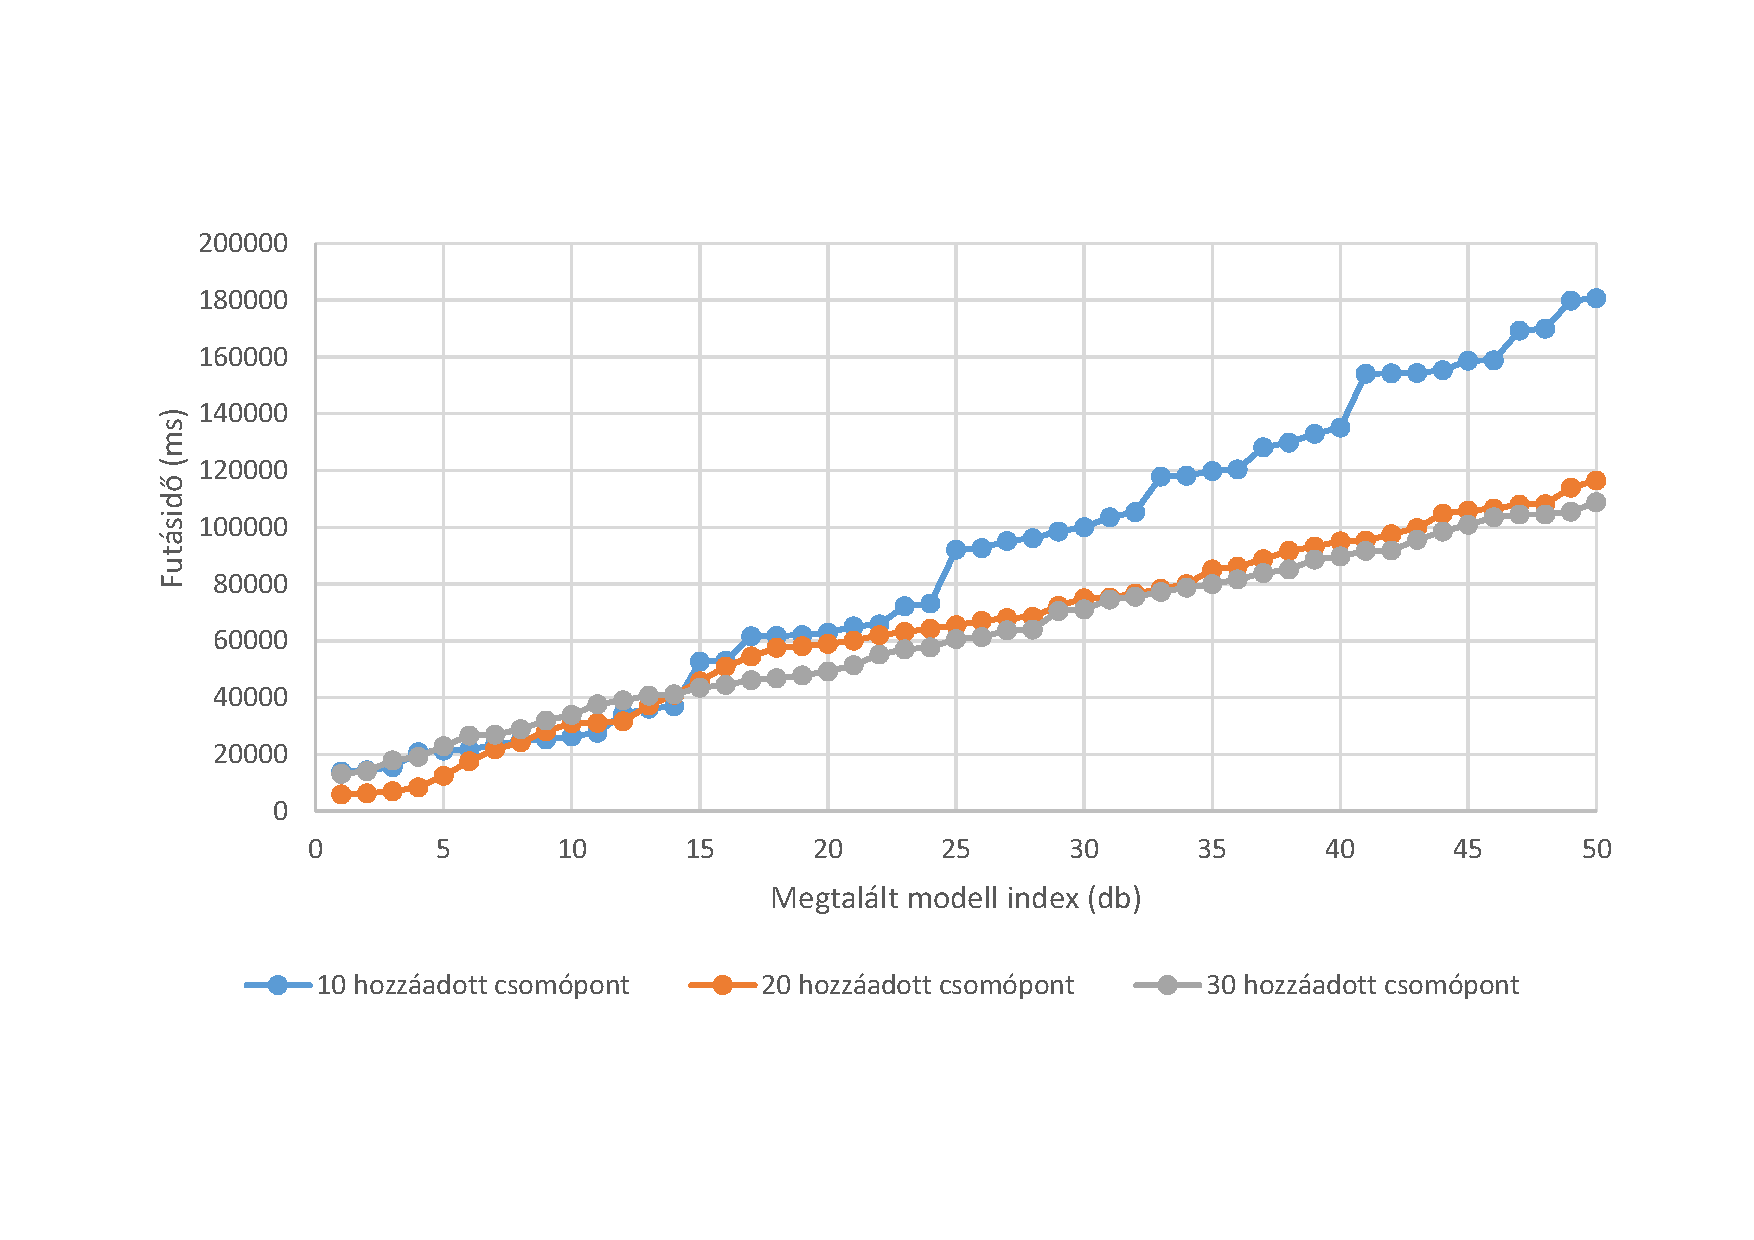
\includegraphics[width=1\textwidth]{figures/statisticsPlottalA}
	\caption{A K2 mérés eredményei}
	\label{fig:AmeresEredmeny}
\end{figure}
                                                                                                                                                                                                                                                                                           
A harmadik kérdésre az M1-es környezetben kerestem a választ. A mérés eredményei \aref{fig:AmeresEredmeny}. ábrán láthatóak. Az 50 darab generált modell megtalálásának ideje nem volt azonos a 10 alkalommal, ezért a 10 érték mediánját kiválasztottam, az ábrán ezeket a medián értékeket jelenítem meg. A 3 méret mérési eredményeit 3 színnel jelöltem. Az ábrán a függőleges tengelyen a futásidő látható milliszekundumban,  a vízszintes tengelyen pedig a létrejött tesztkészlet mérete.  

A három mérés eredményei lineárisak különböző meredekséggel, ez azt jelenti, hogy az egyes modellek megtalálása körülbelül ugyanannyi időt vesz igénybe. Ezen az ábrán is látható, hogy a generátor lassabban végzett a kis modellek megtalálásával mint a nagyokéval. 
                                                                                                               
\textit{Mivel közel lineáris egyenesek születtek a mérés eredményeként, levonható a következtetés, hogy az egyes modelleket körülbelül azonos időközönként találja meg a generátor,  tehát a modellek darabszámának függvényében remekül skálázódik a módszer.}

\section{Diverzitás mérése}


\begin{figure}[htp]
	\centering
	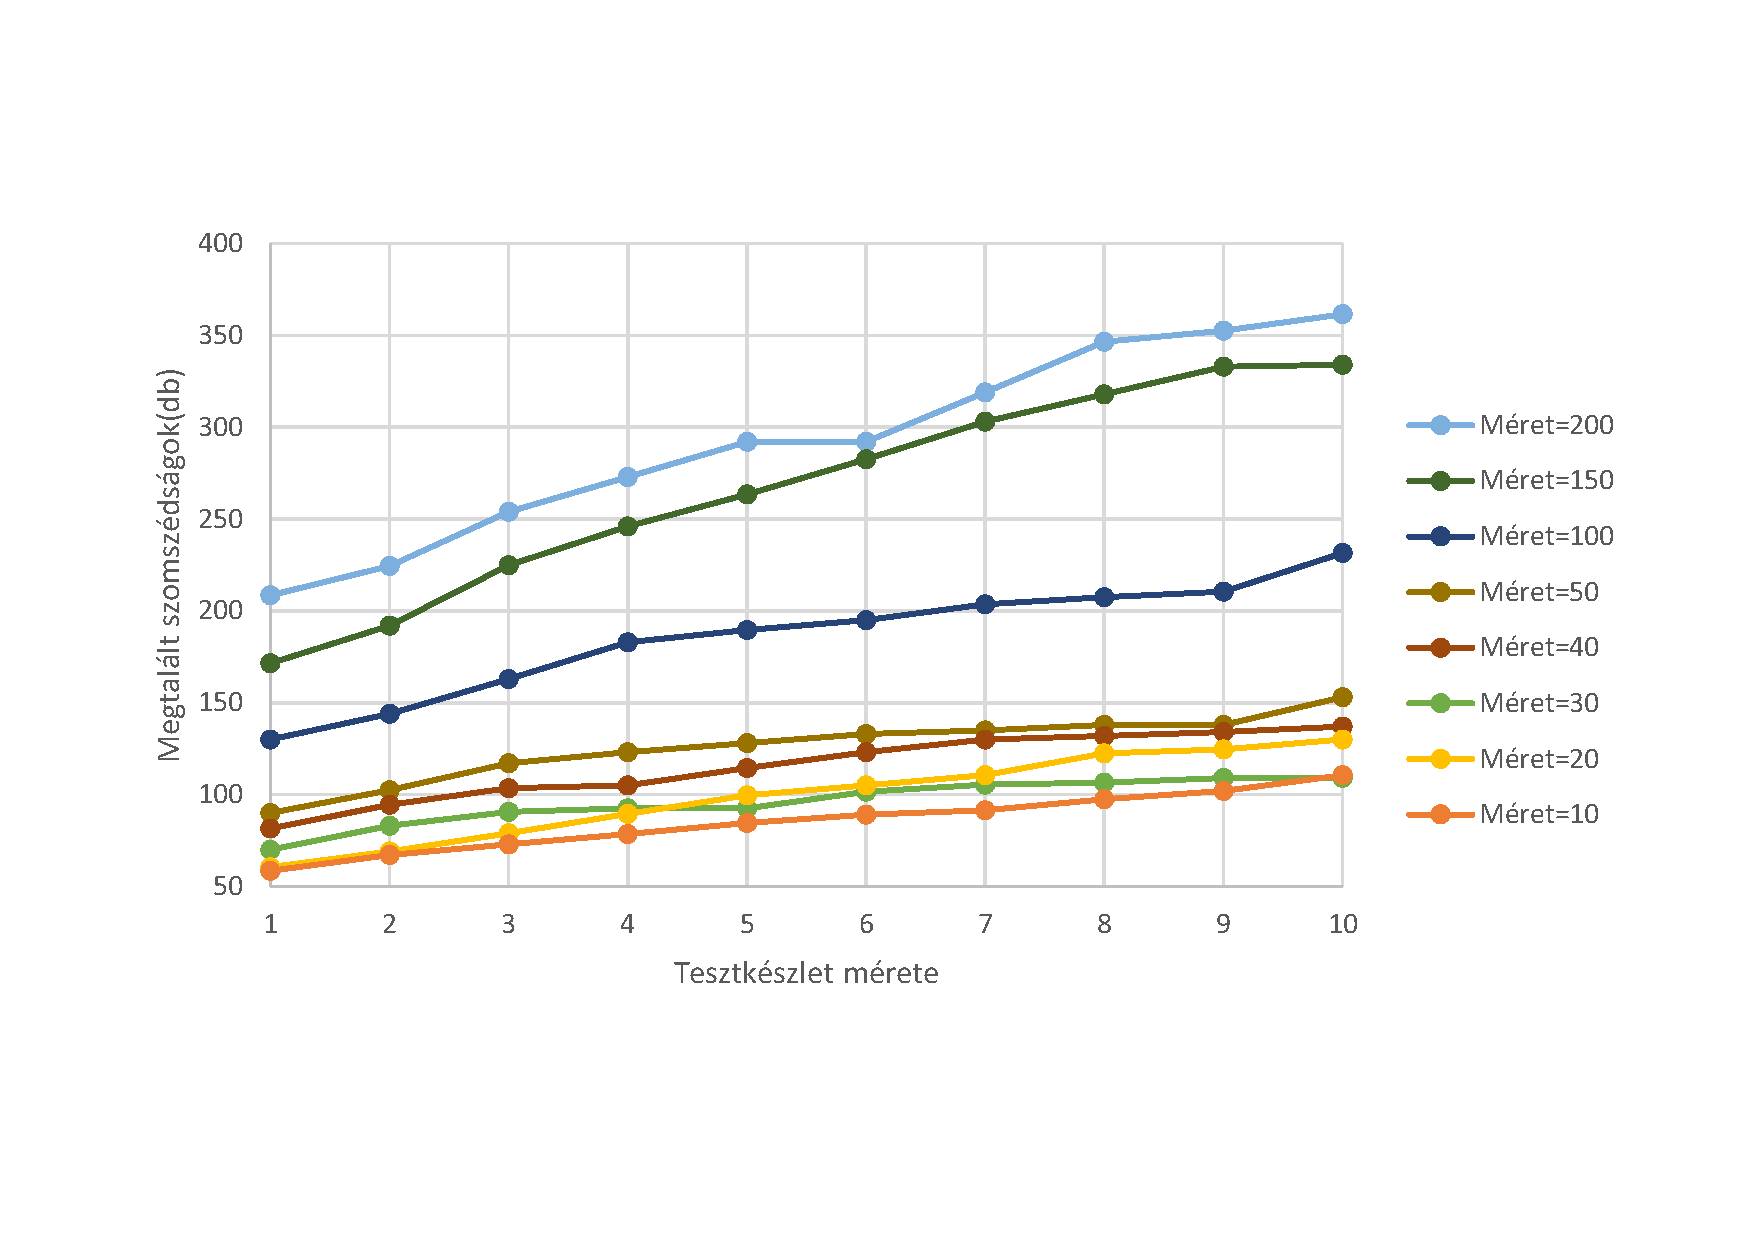
\includegraphics[width=1\textwidth]{figures/diversityB}
	\caption{A K2-es mérés diverzitása}
	\label{fig:BDiversity}
\end{figure}

Az M1 es környezetben végzett mérések során generált lekérdezések diverzitását is kimértem. Ezt szomszédsági formák segítségével tettem. A mérés eredményei \aref{fig:BDiversity}. ábrán láthatóak. Az ábra vízszintes tengelyén a tesztkészlet mérete látható, míg a függőleges tengelyen a megtalált szomszédságok darabszáma 3-as távolságban mérve. Az ábrázolt értékek a különböző minimális hozzáadott elemszámok esetén a 10 mérés mediánját mutatják.

Az ábrán látható, hogy a szomszédságok száma körülbelül lineárisan növekszik az különböző esetekben. A nagyobb lekérdezések esetén azért sokkal több a szomszédság mint a kisebbek esetén, mert ezen az ábrán már a Cypher nyelvre lefordított, nevekkel kitöltött lekérdezések szomszédságait ábrázoltam.

\textit{Levonható tehát a következtetés, hogy a diverzitás kezdetben folyamatosan közel lineárisan növekszik és nagyobb modellek esetén mindig nagyobb diverzitást érünk el.}  

\begin{figure}[htp]
	\centering
	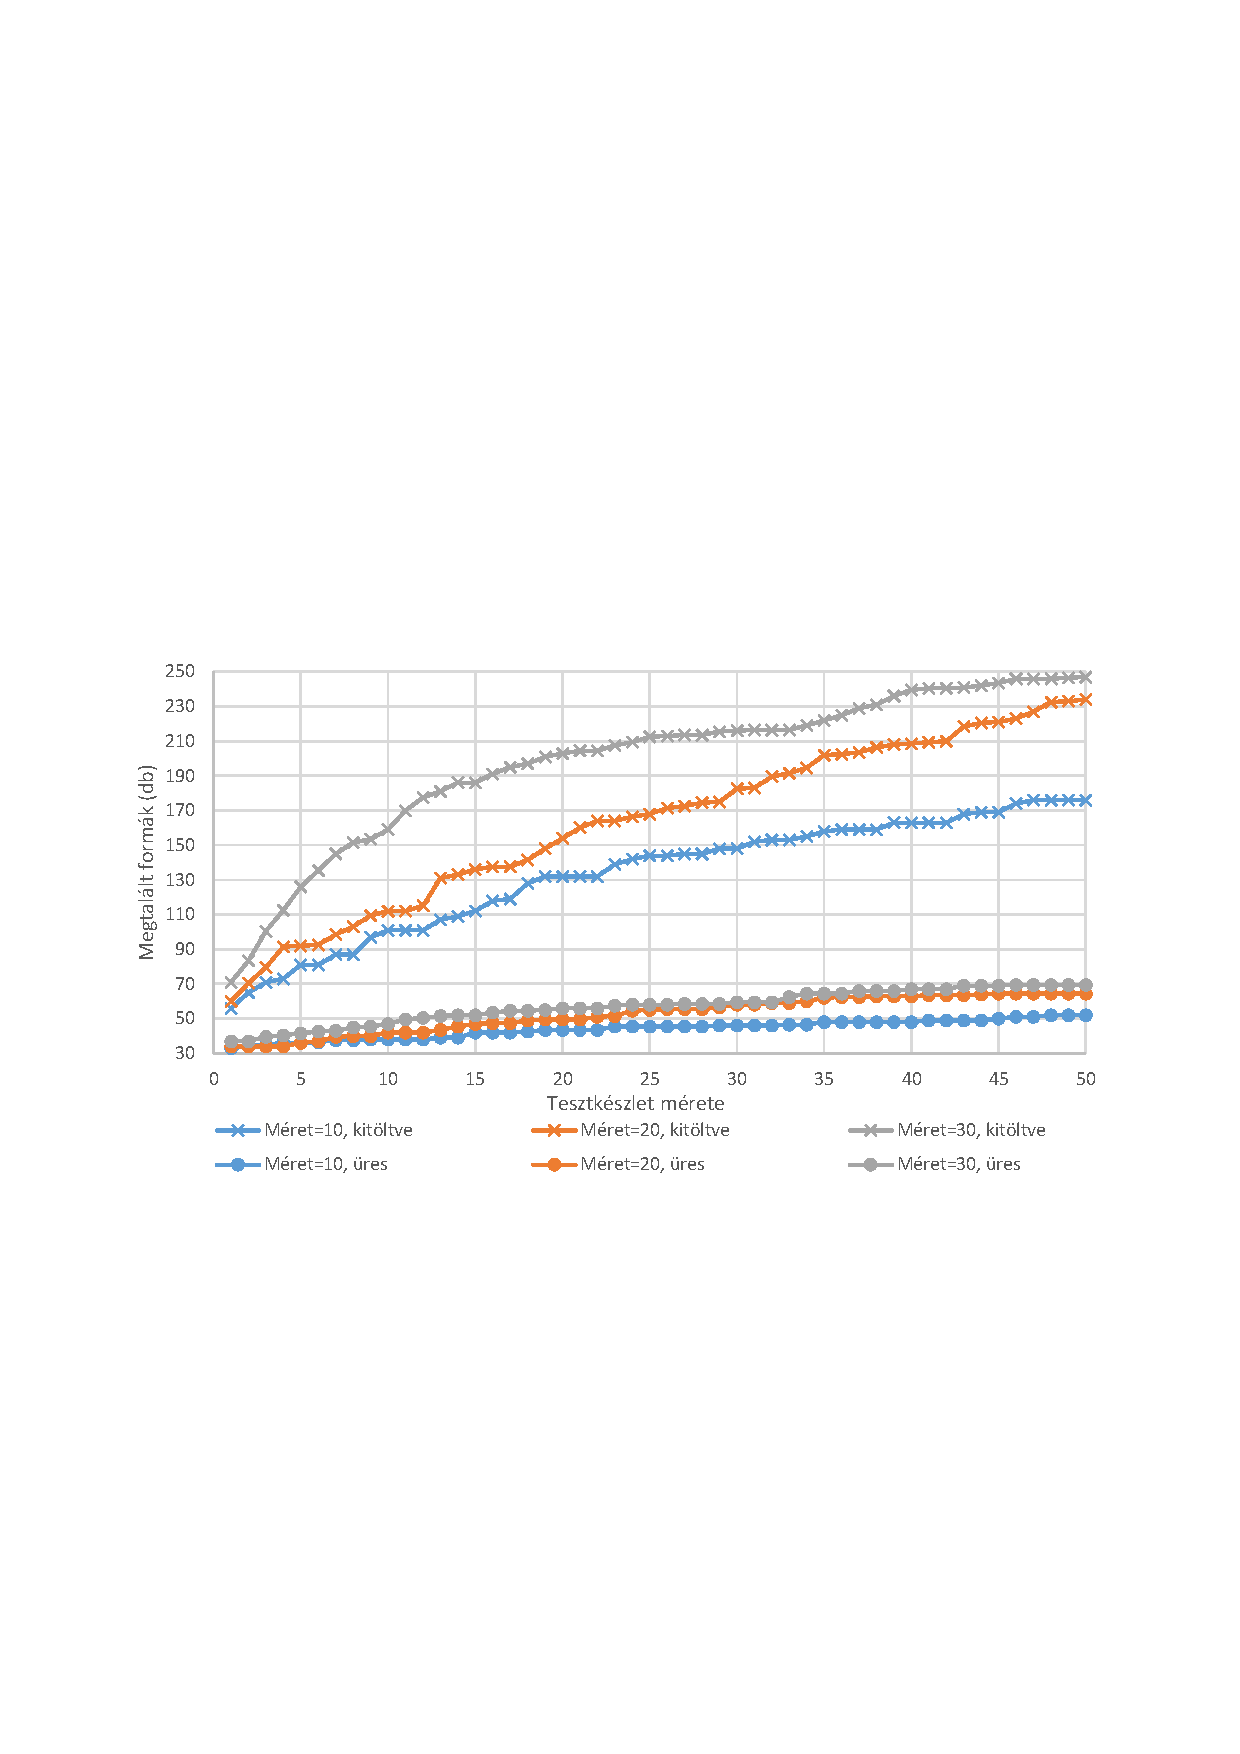
\includegraphics[width=1\textwidth]{figures/diversityA}
	\caption{K3-as mérés diverzitása}
	\label{fig:ADiversity}
\end{figure}

Az M2-es környezetben a lekérdezések és nyers kitöltetlen gráfok diverzitását egyaránt kimértem. A mérés eredményei
\aref{fig:ADiversity}. ábrán láthatóak. Az ábra vízszintes tengelyén a tesztkészlet mérete látható,  a függőleges tengelyen pedig a megtalált szomszédságok darabszáma. Az ábrázolt értékek a 10 elvégzett mérés során kapott értékek mediánjai. 

Az ábrán látható, hogy a kitöltetlen modellek sokkal kisebb diverzitást mutatnak mint a kitöltöttek. Illetve az is látható, hogy a kevés modellnél még lineárissal közelíthető növekedés sok modellnél logaritmikussá alakul. 

\textit{Az általam bevitt diverzitás növelését segítő módszerek tehát hatékonyak, illetve a generálás során a diverzitás folyamatosan növekszik.}

\section{Lekérdezések futásidejének mérése Neo4j adatbázison}

\begin{figure}[htp]
	\centering
	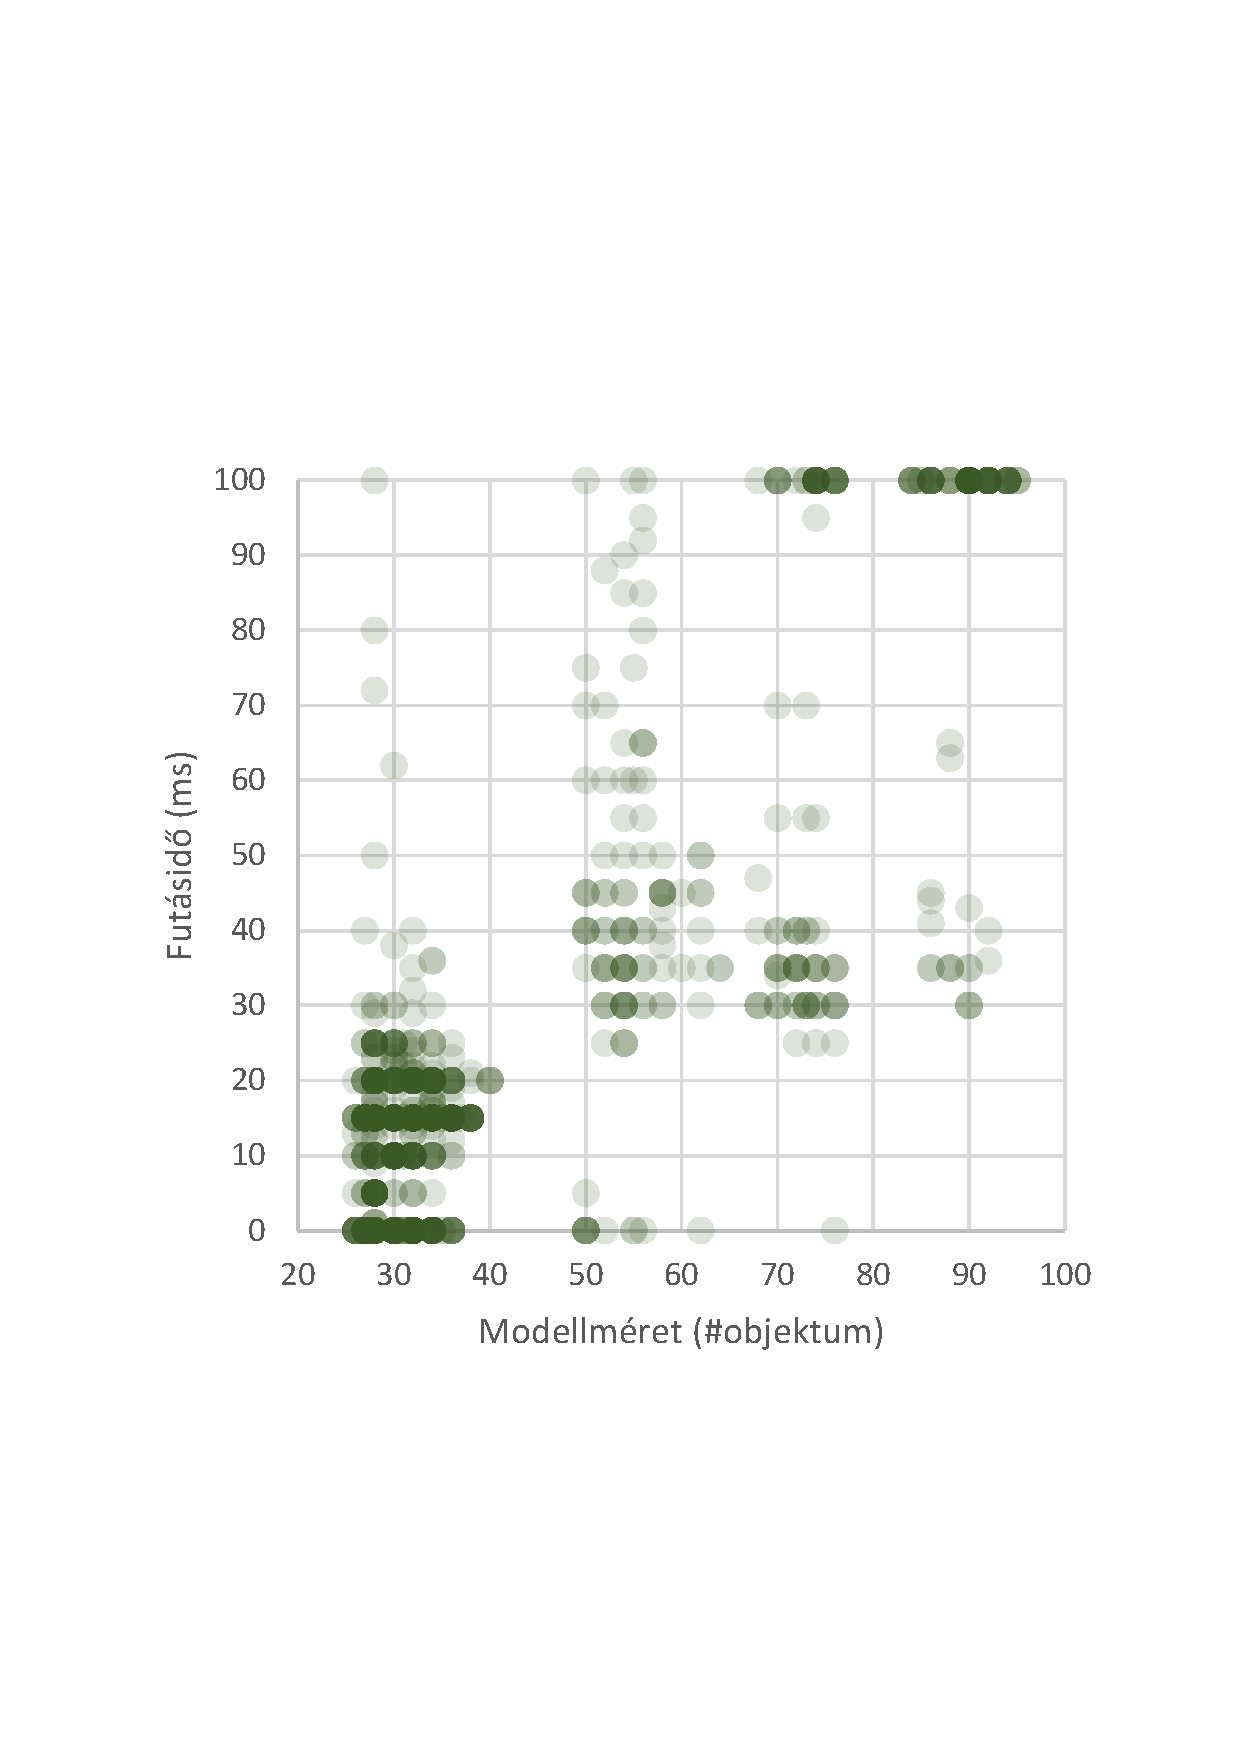
\includegraphics[width=0.6\textwidth]{figures/measurementRuntimeResultNeo4J}
	\caption{Lekérdezéseim futásidejének eredménye}
	\label{fig:Neo4jRuntime}
\end{figure}

Az M2-es környezetben generált lekérdezéseket egy a Train Benchmark által összeállított adatbázison futtattam, amelyben 2024 csomópont és ezek között 5878 kapcsolat volt.
A lekérdezéseket két állapotban futtattam le: (1) attribútumok meghagyásával, és (2) kiszűrésével.
 

Az első futás alkalmával az általam generált lekérdezésekben szereplő attribútum feltételek nem tettek eleget az adatbázisban szereplő attribútum értékeknek, így a legtöbb lekérdezés 0 ms-os eredménnyel nem futott le (ezt ábrán nem szemléltetem).

\textit{Ezzel a méréssel felfedeztük, hogy a Neo4j az attribútumok alapján indexel, és hatékonyan meg tudja válaszolni az ezekkel kapcsolatos lekérdezéseket.}

A második mérés eredményét \aref{fig:Neo4jRuntime}.~ábrán szemléltetem. A pontok az egyes modellekhez tartozó futásidőket jelenítik meg. A vízszintes tengelyen a modellek mérete látható, az alapján számolva hogy hány csomópontból áll az ASG-jük, a függőleges tengelyen pedig a hozzájuk tartozó futásidő. A sötétebb pontok azt jelentik, hogy ott sok egyforma érték született, a halványabbaknál kevesebb. A futásidőt 100-ban maximalizáltam. 

Az ábrán látható, hogy a kisebb modellek kisebb, a közepesek közepes, a nagyok pedig nagyon nagy futásidőt mutatnak, az is látható, hogy míg a kisebb modelleknél volt kevés olyan lekérdezés ami nagyon lassan futott le, addig a nagyobbaknál nem volt olyan ami nagyon gyorsan futott volna le.

 
\textit{Következtetésként levonhatjuk, hogy a generált modellek mérete és a futásidő gyengén korrelál.}

\section{Lehetséges mérési hibák}
\begin{itemize}
	\item Egyetlen esettanulmányon futtattam a méréseket, de ez egy reprezentatív, korszerű, aktívan fejlesztett teljesítmény benchmark, amelyet már több más esettanulmányban is alkalmaztak.\cite{garcia2017stress, bur2018distributed} 
	\item Csak pozitív mintájú lekérdezések generálásával foglalkoztam. Mivel ezek adják az összes lekérdezés alapját a tőlem függetlenül fejlesztett nyelvtanban, jó reprezentatív esetnek számítanak. 
	\item A mérések során mindent csak 10-szer futtattam, de a futásidők és a diverzitások nem mutattak nagy eltéréseket egymástól. A mérési zajt medián számítással mértem ki. A bemelegedés hatását pedig bemelegítő mérések hozzáadásával küszöböltem ki az éles mérések előtt, megvárva a futásidő stabilizálódását.
	\item Bár korrelációt mutat a futásidő és a lekérdezés bonyolultsága ebből egyelőre komolyabb következtetést nem vonhatunk le, ennek értékelése további vizsgálatokat kíván. 	
\end{itemize}




